\documentclass[12pt,letterpaper]{article}
\usepackage[top=2cm, bottom=4.5cm, left=2.5cm, right=2.5cm]{geometry}
\usepackage{fancyhdr}
\usepackage{amsmath}
\usepackage{graphicx}
\usepackage{float}
\setlength{\parindent}{0.0in}
\setlength{\parskip}{0.05in}

\newcommand\course{CSE 417T}
\newcommand\hwnumber{4}                  % <-- homework number
\newcommand\Name{Isabelle Xu and Clayton Knittel}         


\pagestyle{fancyplain}
\headheight 35pt
\lhead{\Name}
\chead{\textbf{\Large Homework \hwnumber}}
\rhead{\course \\ \today}
\lfoot{}
\cfoot{}
\rfoot{\small\thepage}
\headsep 1.5em

\begin{document}

\section*{Problem 1}

\begin{description}
	\item (a) \& (b)

\begin{figure}[H]
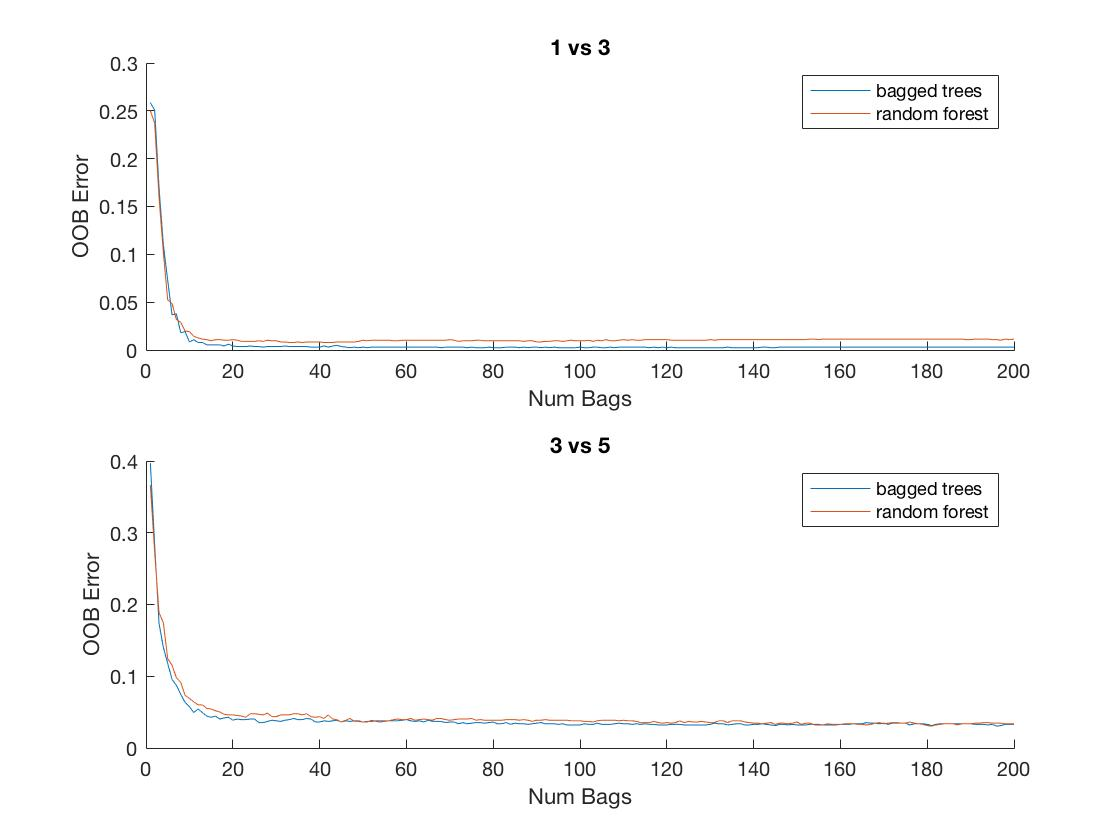
\includegraphics[scale=0.4]{image.jpg} 
\end{figure}

	\item (c) 
\begin{table}[h]
\begin{tabular}{|l|l|l|l|}
\hline
\textbf{Decision Trees} & \multicolumn{2}{l|}{\textbf{Cross Val. Error}} & \textbf{Test Error} \\ \hline
1 vs 3                  & \multicolumn{2}{l|}{0.0090}                   & 0.0163             \\ \hline
3 vs 5                  & \multicolumn{2}{l|}{0.0659}                   & 0.1196	         \\ \hline
\end{tabular}
\end{table}
\begin{table}[h]
\begin{tabular}{|l|l|l|l|}
\hline
\textbf{200 Bagged Trees} & \multicolumn{2}{l|}{\textbf{OOB Error}} & \textbf{Test Error} \\ \hline
1 vs 3                    & \multicolumn{2}{l|}{0.0030}             & 0.0116              \\ \hline
3 vs 5                    & \multicolumn{2}{l|}{0.0338}             & 0.0890              \\ \hline
\end{tabular}
\end{table}
\begin{table}[h]
\begin{tabular}{|l|l|l|l|}
\hline
\textbf{Random Forest} & \multicolumn{2}{l|}{\textbf{OOB Error}} & \textbf{Test Error} \\ \hline
1 vs 3                    & \multicolumn{2}{l|}{0.0090}             & 0.0186              \\ \hline
3 vs 5                    & \multicolumn{2}{l|}{0.0371}             & 0.0767              \\ \hline
\end{tabular}
\end{table}
	\item (d) By definition the differences between all three models is that decision trees model uses only a single tree to learn the data, bagging decision trees utilizes the concept of bootstrap aggregating (combining the predictions of many hypotheses to reduce variance), and random forest utilizes split feature randomization (the ID3 tree building algorithm random chooses a set number of features to select a feature to use when splitting) along with bootstrap aggregating. The results show that 200 bagged decision trees tend to perform better than a single decision tree in classification of digits in both the 1v3 and 3v5 data sets. Because each tree is only looking at some subset of the data, they all will tend to choose different features to differentiate by at each decision point, and thus each will be looking for different aspects of the data points at each step of the decision process when determining which digit it is most likely to be. Therefore, getting a majority vote among the trees is only likely if many different features of a number are like features of a three, not just a few particular ones.
	\\\\As for the differences between 1v3 and 3v5, both plots show very similar behavior except for the fact that 3v5 generally seemed more difficult to learn for all learning models due to how a 3 and a 5 have less distinguishing features between themselves. As a result all the different errors were higher for 3v5 than those of 1v3 all learning models.
	\\\\As we observed from our results, the effects of increasing the number of bags boiled down to a very steep decrease in OOB error before ~10 bags, which then it started to steadily decrease into a plateau ~30 bags. This could be attributed to the fact that OOB error should decease as the number of bags go up as we now probably have a fair sample of the data spread among the trees. For random forest, there is slightly more stochastic decision making on the algorithm's part (split feature randomization), so it takes longer for the error to settle.

\end{description}
\section*{Problem 2}
\begin{description}
	\item (a) \& (b)
\begin{figure}[H]
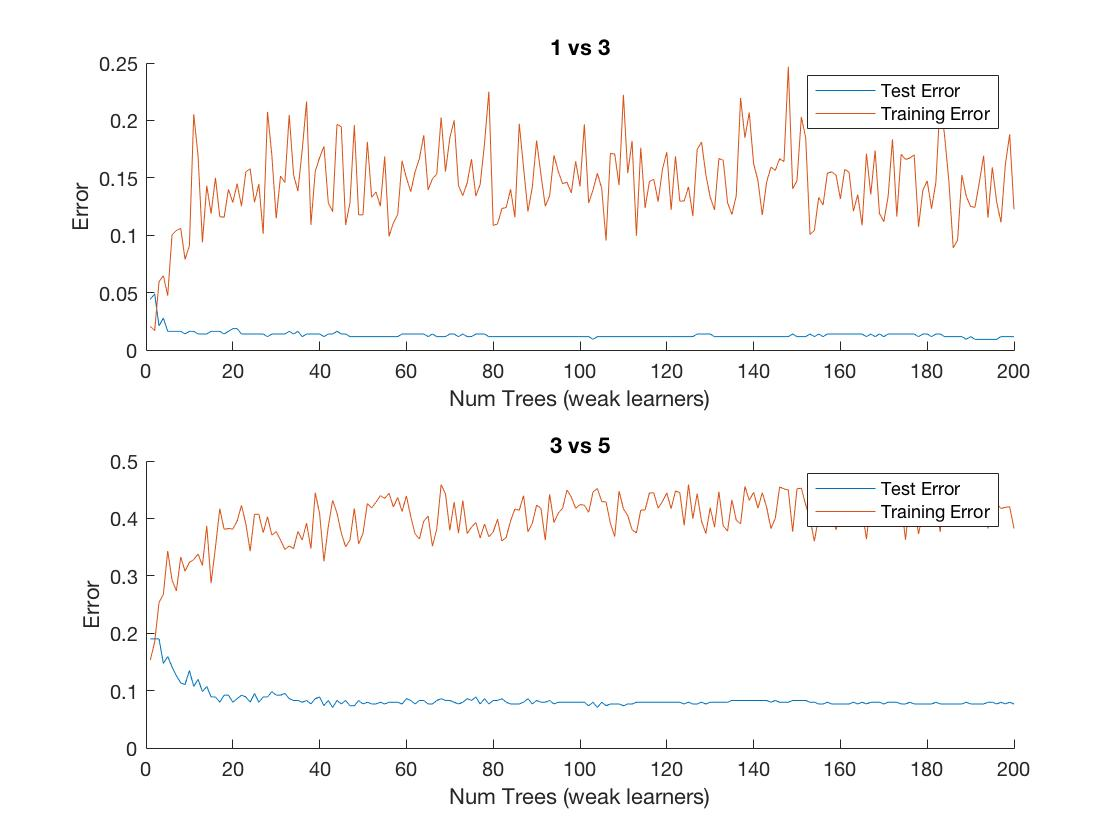
\includegraphics[scale=0.4]{image2.jpg} 
\end{figure}
	\item (c) The differences between 1v3 and 3v5 for the adaboost model is that 1v3 resulted in lower test and training error by a scale of ~0.5.

\end{description}

\end{document}